The training strategy for our segmentation model is composed of four pivotal stages: dataset preprocessing, weak label generation through proxy learning, fine-tuning with gold standard annotations in target learning, and ensemble learning. A detailed elaboration of these stages follows:

\section{Dataset Preprocessing}

Our exploratory data analysis unveiled that non-background voxels constitute only a minor proportion of the overall MRI volume. Consequently, they might not impart sufficient information to enable effective learning by the segmentation model. To rectify this issue, we exploit the provided centreline coordinates of the terminal ileum to define the bounding box encompassing the T.I. region. The original volume is then cropped to this reduced version for implementing the baseline, and the bounding box information is introduced for refining the weak labels with the pre-trained SAM model, which significantly curtailing data complexity and ensuring that the retained labelled voxels play a crucial role in facilitating model learning.

Prior to initiating training, the dataset must be restructured into a specific format as stipulated by nnU-Net \cite{isensee2021nnu}. As per this convention, the name of each dataset should adopt the form \texttt{`Dataset<ID>\_<NAME>'}. Moreover, each dataset is accompanied by a configuration file providing essential metadata, such as the modalities of MRI imaging employed for each patient, along with the semantic interpretation of the segmented labels within the ground truth results. The images and corresponding labels assigned for training are situated within the dataset folder, separated into distinct directories: \texttt{`imagesTr'} and \texttt{`labelsTr'}. Note that we treated coronal and axial T2 as two separate datasets to complete the segmentation task. 

Upon successful conversion of the dataset, nnU-Net initiates preprocessing, modifying images to different dimensions and resolutions optimised for ensemble model training. Concurrently, a unique \textbf{`dataset fingerprint'} is derived, earmarked for subsequent hyperparameter tuning. With these preparatory steps completed, the preprocessed data is primed for the ensuing proxy learning task.

By adopting such a meticulous approach to data preprocessing, we ensure that our model is furnished with optimally structured data, thereby enhancing its capacity to learn effectively from the available information and generate accurate segmentations.

\section{Baseline Implementation}

Building upon precedent research, we've formulated a baseline model that adheres to a systematic and robust methodology. This model lays the groundwork for further enhancement and modifications later in our project:

Our first step involves the application of 3D Simple Linear Iterative Clustering (SLIC) superpixel segmentation on the cropped Region of Interest (ROI). This task serves to generate a weak mask that becomes instrumental in our proxy learning stage. To ensure the successful execution of this step, we identify the superpixels situated on the centreline of the terminal ileum, leveraging provided centreline coordinates. Subsequently, the segmented superpixels are relabelled to binary labels, as it realigns output with our project objectives.

Upon generation of the initial segmentation, we confront the potential issue of hole or tube-like structures within the segmented supervoxels. These irregularities can disrupt the continuity of the terminal ileum representation. Therefore, our process incorporates the use of a voting iterative binary hole filling algorithm in conjunction with morphological hole closing to create a more refined segmentation.

With the generation of weak masks accomplished, we proceed to train our proxy model. Furthermore, a second iteration of training is conducted, this time deploying the proxy model on fully-annotated data to obtain the final segmentation model. Additional aspects of the training process, along with the ensembling strategy employed to derive the final model, will be elaborated in the ensuing sections.

\section{Model Training}
As we step into our process, our attention is directed towards the pivotal stage of model training. This stage is characterised by an enriched proxy learning strategy, where we replace the initial unsupervised 3D SLIC-based weak mask generation with a more sophisticated tool: MedSAM. Additionally, the training and evaluation phases are designed to optimise model performance, incorporating cross-validation and ensemble learning methods. Below, we elaborate on these key aspects:

\begin{itemize}
\item \textbf{MedSAM Application}:
In this subsection, we discuss in detail how we leverage MedSAM for generating high-quality weak masks, elucidating its superior capabilities in the context of medical image segmentation and its specific role in enhancing our model learning trajectory.

\item \textbf{Dataset Partitioning}:
Here, we explain how we divide our dataset into training and testing sets using an 80/20 ratio. We provide rationale for this split and discuss how it ensures a robust and unbiased evaluation of our model performance.

\item \textbf{Training Pipeline}:
Our multifaceted training pipeline starts with a two-phased approach. Initially, we train a proxy model on weak masks generated by MedSAM. This is followed by further training on 80\% of the fully annotated data, maximizing learning from both weakly and fully annotated data sets.

To ensure model robustness, a 5-fold cross-validation method is integrated during training to mitigate overfitting risks. Furthermore, our pipeline supports different configurations, which includes 2D and 3D variants of data, loss function adjustments, and variations in training optimisers and learning rates.

The final aspect of our pipeline is ensemble learning, utilized to aggregate models across different folds and configurations, thereby generating our target model. The collective operation of these facets is meticulously designed to bolster our model performance in diverse scenarios.

\item \textbf{Inference}:
In this final stage, we delve into the utilization of the trained model for making inferences. Our focus lies in outlining the procedural aspects of applying the model to new and unseen data, thus generating predictive outcomes that form the basis for the subsequent comprehensive evaluation of our model performance. The evaluation process, with a detailed quantitative analysis, will be discussed extensively in the following chapter.
\end{itemize}

Through this comprehensively planned model training phase, we aim to build a proficient terminal ileum segmentation model that not only learns effectively from our data but also showcases robust performance across varying scenarios.

\subsection{Refining Weak Masks with MedSAM}

Enhancing the quality of our weak masks forms an integral part of our methodology. For this, we leverage a modern mask generation technique - MedSAM, a variant of the SegmentAnything Model. Being tailored for medical images, MedSAM enables the creation of refined, granular weak masks, thereby setting the stage for improved segmentation results.

The process unfolds with our preprocessed images being introduced to MedSAM. Traditional methods pale in comparison to this sophisticated tool which, equipped with cutting-edge AI algorithms, excels in discerning the distinct characteristics intrinsic to medical images. The outcome is a granular segmentation that far surpasses the precision achievable with conventional models. A noteworthy augmentation to our preprocessing phase includes the inclusion of the extracted ROI along with the bounding box of centreline coordinates specific to the T.I. region. Evidence from Huang et al., 2023 \cite{huang2023segment}, suggests that such enrichment significantly amplifies the quality of the resulting weak mask. For images lacking provided centerline information, we elect to exclude them from the dataset, thus ensuring a consistent and reliable source of data for our methodology.

Once these refined weak masks are generated, we align the mask labels to the binary format, thereby syncing it with our project objectives. Subsequently, these weak masks are employed during the proxy learning phase of our training pipeline.

The introduction of MedSAM into our pipeline marks a pivotal step towards superior segmentation outcomes - the refined masks open up enhanced learning avenues for our model, laying a solid foundation for further advancements in terminal ileum segmentation.

\subsection{Executing Dataset Partitioning}

The partitioning of our dataset into training and testing sets plays a crucial role in our model development. This strategy helps ensure that the model performance is assessed on new, unseen data, establishing a reliable measure of its predictive capabilities.

Our approach involves a partitioning of the dataset into an 80/20 ratio. Prior to this division, we shuffle the dataset to randomise the order of samples, ensuring an unbiased representation in both the training and testing sets. Subsequently, the first 80\% of these randomized samples form our training set while the remaining 20\% are reserved for testing.

The reason of using such ratio is because it is widely revered in the field of machine learning, serves to strike a balance between providing sufficient data to nourish the model's learning journey and withholding a substantial portion for an authentic evaluation of its performance. This balance becomes particularly crutial when navigating through scenarios characterised by a limited dataset, such as ours.

This cautious allocation of data equips us with a model that's not only well-trained but also rigorously tested for its predictive performance, thereby strengthening our confidence in its segmentation ability.

\subsection{Establishing the Training Pipeline}
This subsection outlines on principal components of our training pipeline, including the deliberate choices and reasonings behind formulating the loss function, selecting the optimiser and determining the learning rate. Additionally, a two-phased training approach is proposed with the key components collevtively to ensure the model's capability to learn efficiently, navigate an optimised prediction path and deliver robust T.I. segmentation.
\subsubsection*{Loss Function Formulation}
Guiding the learning trajectory of our model during training is an elegantly designed loss function. Particularly, we harness nnU-Net's unique blend of cross-entropy and Dice losses \cite{drozdzal2016importance}, expressed as:

\[
\mathcal{L} = \mathcal{L}_{CE} + \mathcal{L}_{Dice}
\]

For our specific use-case, this composite loss function manifests into a binary form, simplifying to a binary cross-entropy loss defined as:

\[
\mathcal{L}_{CE} = \sum_{i}^{N}\left(y_{i}\log o_{i} + (1 - y_{i}) \log (1 - o_{i})\right)
\]

In this equation, \(y_{i} \in \{ 0, 1 \}\) symbolizes the ground truth label for the \(i\)-th instance, while \(o_{i} \in \left[0, 1\right]\) represents the corresponding softmax probability for the given label \(y_{i}\).

Complementing this, the Dice loss is articulated as:

\[
\mathcal{L}_{Dice} = -\frac{2\sum_{i}^{N}o_{i}y_{i}}{\sum_{i=1}^{N}\left(o_{i} + y_{i}\right)}
\]

Here, \(N\) encapsulates the total number of pixels present in the training batch.

The careful orchestration of these two components within the loss function empowers our model to effectively traverse the complex learning landscape, ultimately optimising its performance in terminal ileum segmentation.

\subsubsection*{Optimiser Selection}

In constructing an effective training strategy for our model, we deploy Stochastic Gradient Descent (SGD) as the principal optimizer, supplemented by a Nesterov momentum set to 0.99.

This process can be imagined as an expert guide traversing complex terrain in search of the lowest point or valley - an analogy for the optimal solution that minimizes error. In this context, SGD serves as our skilled explorer, persistently heading towards the steepest downward gradient in pursuit of the valley.

However, as any experienced guide would attest, the steepest descent does not necessarily lead to the lowest valley due to potential undulations and variations in the terrain further ahead.

Addressing this challenge is the role of the Nesterov momentum. It equips our guide with a metaphorical telescope, allowing for a foresighted view of the landscape along the current path before finalising the next step. This foresight permits more informed decisions that consider the overall landscape, rather than just the immediate surroundings.

This stands in contrast to the classical momentum method, which can be considered as a hiker who relies solely on their current position and pace to determine their next step without any foresight or scouting tools. A intuitive illustration of the difference between the effect of classical and Nesterov Momentum is shown in \autoref{fig:nesterov} \cite{lectures16:online}.

\begin{figure}[htp]
    \centering
    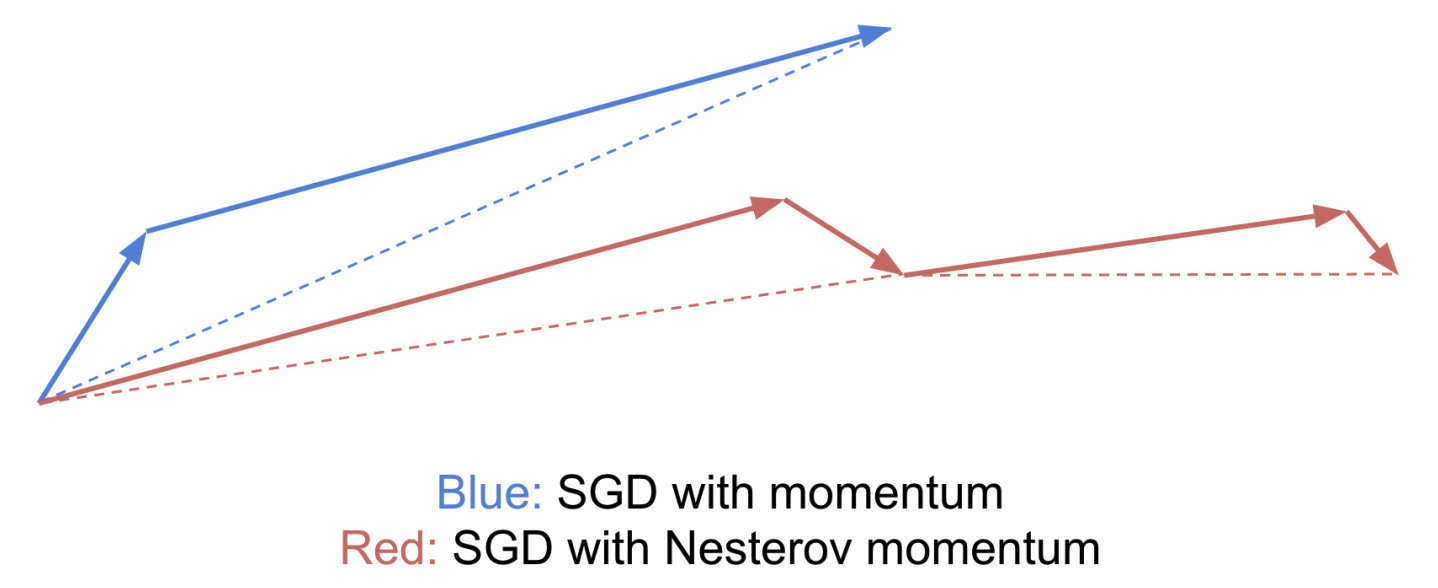
\includegraphics[width=0.8\textwidth]{./figures/nesterov.png}
    \caption{Nesterov momentum}
    \label{fig:nesterov}
\end{figure}

Employing Nesterov momentum with our SGD optimizer consequently enables a quicker and more precise journey to the `valley' or optimal solution, ensuring our model learns both effectively and efficiently from our data.

To illustrate this concept more clearly, \autoref{alg:sgd-nesterov} outlines this process in details:
\begin{algorithm}[htp]
\caption{SGD enhanced with Nesterov Momentum}\label{alg:sgd-nesterov}
\begin{algorithmic}[1]
\Require Initial learning rate \(\eta\), momentum \(\beta\)
\Require Initial parameter \(\mathbf{\theta_{0}}\), initial velocity vector \(\mathbf{v_{0}}\)
\While{not reaching stopping criteria}
\item Draw one batch with \(m\) samples \({ x^{(1)}, \ldots , x^{(m)} }\) with corresponding \(y^{(i)}\)
\item Temporarily update the parameter: \(\tilde{\mathbf{\theta_{t}}} \leftarrow \mathbf{\theta_{t}} - \beta \mathbf{v_{t}}\)
\item Compute the gradient at the adjusted point:
\[
\mathbf{g_{t}} \leftarrow \nabla_{\tilde{\mathbf{\theta_{t}}}}\sum_{i}\mathcal{L}(f(x^{(i)}; \tilde{\mathbf{\theta_{t}}}), y^{(i)})
\]
\item Refresh the velocity: \(\mathbf{v_{t+1}} \leftarrow \beta\mathbf{v_{t}} + \eta \mathbf{g_{t}}\)
\item Update the parameter: \(\mathbf{\theta_{t + 1}} \leftarrow \mathbf{\theta_{t}} - \mathbf{v_{t + 1}}\)
\EndWhile
\end{algorithmic}
\end{algorithm}

In more technical terms, the Nesterov momentum method facilitates accelerated learning relative to traditional methods. This acceleration is of crucial strategic value, as it leads to significant time and resource efficiencies, thereby boosting the progression of our model into a highly competent predictive tool in a shorter span.

\subsubsection*{Learning Rate Determination}
The learning rate is a crucial factor in optimising our model, which guides the magnitude of updates made to learnable parameters during each iteration. We have set an initial learning rate of 0.01 to balance by ensuring that our model learns at a steady pace without missing out or skipping over essential information.

The key characteristic of our approach, however, is that our learning rate is not constant — it gradually decreases as training progresses. This strategy, known as learning rate annealing or decay, plays a essential role in optimising our model performance.

As the training advances, model parameters tend to converge towards an optimal solution. Here, making large adjustments is not ideal because it might cause the parameters to oscillate around (or overshoot) the desired optimum. To address this issue, we decrease the learning rate across iterations, encouraging smaller steps when we are presumably closer to the optimum, and therefore enhancing the model performance over time.

We employ a learning rate scheduler that uses a polynomial function determined by the total number of training iterations. The decaying learning rate, \( \eta_{t} \), is computed by:
\[
\eta_{t} = \eta_{0}(1 - \frac{t}{N})^{0.9}
\]

Here, \( \eta_{0} = 0.01 \) is the initial learning rate, \( t \) stands for the current iteration count, and \( N \) represents the total iterations.

By carefully managing the learning rate via this method, we ensure that our model can adapt effectively across training steps, continually refining its performance with each iteration.

\subsubsection*{Two-phased training}
Our training pipeline adopts a two-phased strategy, heavily leveraging the loss function, optimizer, and learning rate detailed prior.

In the first phase, the proxy model is trained using the generated weak mask over 200 epochs, reserving 20\% of the training data for validation. This process utilises a SGD optimiser with Nesterov momentum and an initial learning rate of 0.01 with our proposed strategy of learning rate decay. Upon completion of this preliminary phase, nnU-Net collates the validation results and combines them with pre-extracted dataset fingerprints to finalise the optimal hyperparameter combination for the proxy model.

The subsequent phase fine-tunes the proxy model on fully annotated images across 50 epochs. A 5-fold cross-validation along with the same optimisation settings as the previous phase is used to ensure a effective learning trajectory. Notably, only 80\% of the fully annotated data feeds into this stage, preserving 20\% of the data and their corresponding ground truth segmentations for ultimate evaluation.

This two-phase strategy remains adaptable to varied data configurations, accommodating differences in image dimensions and resolutions, while seamlessly integrating with both 2D and 3D full-resolution data. We ensure each model concludes its training, strategically combine predictions on unseen gold standard data to determine the final output.

The selection of the final model is guided by cross-validation performance. Depending on the outcomes, the final model could either be a single best-performing model or an ensemble of models trained across different folds. Throughout this meticulously planned two-phase training, our objective remains consistent: To create a proficient model capable of delivering exceptional terminal ileum segmentation.

\subsection{Executing the Inference Process}

Once the optimal model is determined, we are equipped to introduce unseen, pre-processed data into the nnU-Net framework. This enables us to generate straightforward predictions. However, it is important to highlight several points that characterise this predictive phase.

In alignment with nnU-Net's patch-based training procedure, inference also adopts a patch-based methodology. Each image is divided into smaller sub-images or `patches', and it is upon these patches that our model bases its predictions. Nevertheless, another worth-mentioning point is that the model precision tends to decrease towards the edge of these patches. Consequently, when generating predictions, the model attributes greater significance to the voxels situated near the centre of the patch as compared to their edge-located counterparts. This strategy ensures a notably higher prediction quality upon aggregating the predictions across all patches.

Upon the completion of the model prediction, a common practice is to apply post-processing to the generated predictions. Post-processing is often employed based on connected components to enhance image segmentation, such as organs. This approach typically centres on disregarding smaller, potentially insignificant elements and laying emphasis on the most expansive interconnected region to mitigate the probability of false positives.

Exemplifying this philosophy, nnU-Net systematically utilises the implications of omitting these smaller entities on the model performance, employing cross-validation results as a reference metric. Initially, each foreground class is treated as a singular entity. If the constraint to the largest region increases the average foreground Dice coefficient without diminishing any class-specific coefficients, then this method emerges as the preliminary post-processing step. Subsequent to the outcome of this stage, nnU-Net determines whether the same method requires application to individual classes.

This sophisticated, multi-faceted approach to inference empowers us to maximise the accuracy, reliability, and clinical relevance of our terminal ileum segmentation predictions.